% example tikz figure

\documentclass{article}
\usepackage{amsmath}
\usepackage{amsfonts}
\usepackage{tikz}
\usetikzlibrary{arrows,shapes,positioning,shadows,trees}


\begin{document}

\begin{tikzpicture}
    % draw axis with arrows, length 5
    \draw[->] (-3,0) -- (5,0);
    \draw[->] (0,-3) -- (0,5);

    % circle centered at point (2,0) radius 2
    \draw (2,0) circle (2);

    \draw[-] (0,0) -- (2,3);
    % label the angle to x-axis
    \draw[-] (0.5,0) arc (0:56.3:0.5);

    % label (2,3) as z = r e^{i \theta}
    \node[right] at (2,3) {$z = r e^{i \theta}$};

    % draw arbitrary arc from (2,0), to (2,3), not straight line, and label the arc as gamma_1
    \draw [-] plot [smooth, tension=1] coordinates {(2,0) (2.5,1) (2,3)};

    \node[right] at (2.6,1.5) {$\gamma_1$};

    \node[below] at (2,0) {$i$};

    % \draw [->] (2,0) arc (-20:-160:2);
    % \draw [->] (-1.75,0) arc (180:80:3.1);
    \draw [-] plot [smooth, tension=1] coordinates {(2,0) (0,-2) (-2,0) (0,3) (2,3)};

    \node[above left] at (-2,0) {$\gamma_2$};
\end{tikzpicture}

\begin{tikzpicture}
    \node (a) at (0,0) {
        \begin{tikzpicture}
            % three circles centerd at (0,0), radius 1, 2, 3
            \draw (0,0) circle (1);
            \draw (0,0) circle (2);
            \draw (0,0) circle (3);

            % pick theta=pi/6 at radius 2
            \draw[-] (0,0) -- (1.732,1);
            % label on top right z_0
            \node[above right] at (1.732,1) {$z_0$};
            % go pick the mirror point
            \draw[-] (0,0) -- (-1.732,-1);

            % label O with (0,0) filled circle
            \node[fill,circle,inner sep=1pt,label=below right:$O$] at (0,0) {};
            \node[below right] at (-1.732 * 3 / 4, - 3 / 4) {$\rho$};

            \draw[-] (0,0) -- (-1.732 / 2, 0.5);
            % as above, label this ar r
            \node[below] at (-1.732 / 4, 0.25) {$r$};

            \draw[-] (0,0) -- (-0.5 * 3, 1.732 * 3 / 2);
            \node[right] at (-0.5 * 3 / 2, 1.732 * 3 / 4) {$1$};
        \end{tikzpicture}
    };


    \node (b) at (10,0) {
        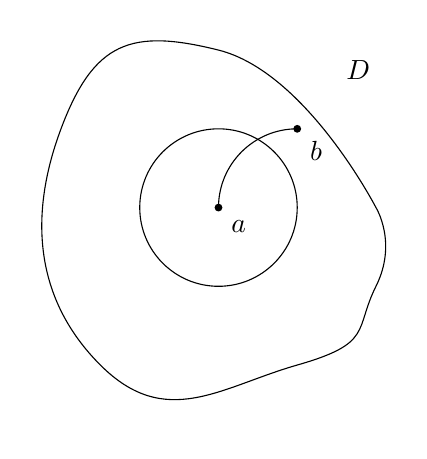
\begin{tikzpicture}
            \draw (0,0) circle (1);
            \draw [-] plot [smooth, tension=1] coordinates {(2,0) (0,2) (-2,1) (-1.5,-2) (1,-2) (2,-1) (2,0)};

            % label origin as a
            \node[fill,circle,inner sep=1pt,label=below right:$a$] at (0,0) {};

            \node[fill,circle,inner sep=1pt,label=below right:$b$] at (1,1) {};

            % arc from (0,0) to (1,1) with center (0,1)
            \draw[-] (0,0) arc (180:90:1);
            \node[above right] at (1.5, 1.5) {$D$};
        \end{tikzpicture}
    };

    \node(c) at (10, -5) {$\mathbb C$};

    % line from a to b
    \draw[->] (a) -- (b);
    % label the line at top: $\Phi^{1-1}$
    \node[above] at (5,0) {$\Phi^{1-1}$};

    % line from a to c
    \draw[->] (a) -- (c);
    % label the line at bottom: $P\cdot \Phi$
    \node[below] at (6,-3.5) {$P\cdot \Phi$};

    % line from b to c
    \draw[->] (b) -- (c);
    \node[right] at (10, -3.5) {$P(z)$};
\end{tikzpicture}
\end{document}